\section{Verwendete HDR Maps} % (fold)
\label{sec:verwendete_hdr_maps}

	\renewcommand{\arraystretch}{1.3}
	\begin{table}[H]
		\begin{tabularx}{\textwidth}{p{0.35\textwidth}p{0.60\textwidth}}
			\hline
			\textbf{Bild} & \textbf{Daten} \\
			\hline
			\hline \\

			\raisebox{-0.8\totalheight}{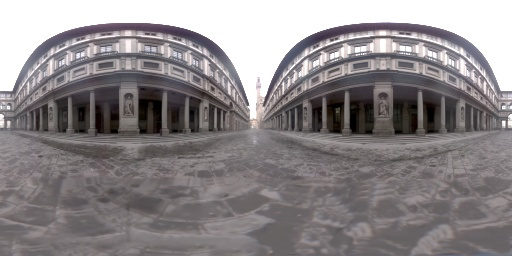
\includegraphics[width=0.3\textwidth]{pic/hdr-uffizi_gallery.jpg}} & \parbox[t]{0.64\textwidth}{\textbf{\enquote{Uffizi Gallery}:} \bigskip\\ Uffizi Gallery, Italy \bigskip\\ Quelle: \cite{hdr-gallery}} \\
			\\
			\hline \\

			\raisebox{-0.8\totalheight}{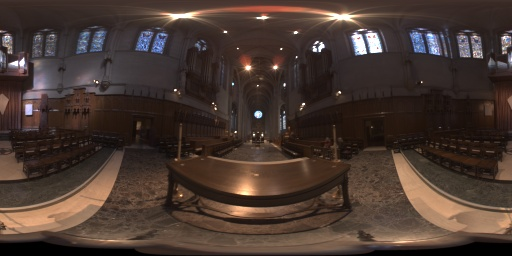
\includegraphics[width=0.3\textwidth]{pic/hdr-grace_cathedral.jpg}} & \parbox[t]{0.64\textwidth}{\textbf{\enquote{Grace Cathedral}:} \bigskip\\ Grace Cathedral, San Francisco, California \bigskip\\ Quelle: \cite{hdr-gallery}} \\
			\\
			\hline \\

			\raisebox{-0.8\totalheight}{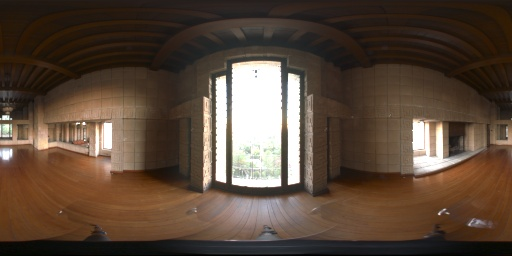
\includegraphics[width=0.3\textwidth]{pic/hdr-ennis-brown_house.jpg}} & \parbox[t]{0.64\textwidth}{\textbf{\enquote{Ennis-Brown House}:} \bigskip\\ Ennis-Brown House, Los Angeles, California \bigskip\\ Quelle: \cite{hdr-gallery}} \\
			\\
			\hline \\

			\raisebox{-0.8\totalheight}{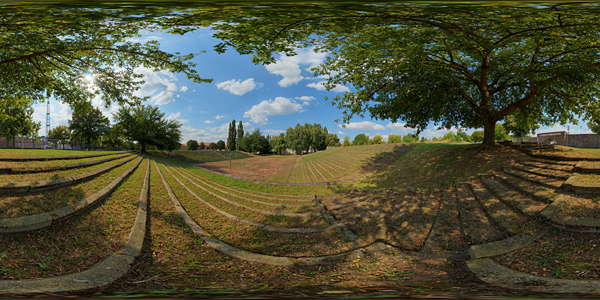
\includegraphics[width=0.3\textwidth]{pic/hdr-basketball_court.jpg}} & \parbox[t]{0.64\textwidth}{\textbf{\enquote{Basketball Court}:} \bigskip\\ Quelle: \cite{hdr-basketballcourt}} \\
			\\
			\hline \\

			\raisebox{-0.8\totalheight}{
\includegraphics[width=0.3\textwidth]{pic/hdr-sky_10.png}} & \parbox[t]{0.64\textwidth}{\textbf{\enquote{Sky 10}:} \bigskip\\ Quelle: \cite{hdr-skies}} \\
			\\
			\hline \\

			\raisebox{-0.8\totalheight}{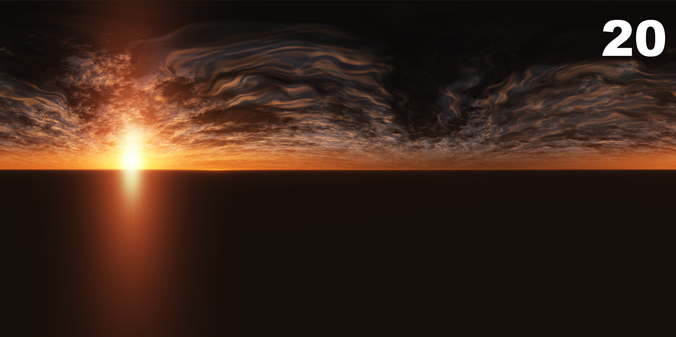
\includegraphics[width=0.3\textwidth]{pic/hdr-sky_20.png}} & \parbox[t]{0.64\textwidth}{\textbf{\enquote{Sky 20}:} \bigskip\\ Quelle: \cite{hdr-skies}} \\
			\\
			\hline

		\end{tabularx}
	\end{table}

% section verwendete_hdr_maps (end)